% Modified based on Xiaoming Sun's template
\documentclass{article}
\usepackage{amsmath,amsfonts,amsthm,amssymb}
\usepackage{ctex}
\usepackage{setspace}
\usepackage{fancyhdr}
\usepackage{lastpage}
\usepackage{extramarks}
\usepackage{chngpage}
\usepackage{soul,color}
\usepackage{graphicx,float,wrapfig}
\usepackage{enumitem}
\usepackage{array}
\usepackage{listings}
\usepackage{xcolor}
\lstset{
  language = python, numbers=left, 
         numberstyle=\tiny,keywordstyle=\color{blue!70},
         commentstyle=\color{red!50!green!50!blue!50},frame=shadowbox,
         rulesepcolor=\color{red!20!green!20!blue!20},basicstyle=\ttfamily
}
\renewcommand{\d}{\mathrm{d}}
% \renewcommand{\p}{\partial}
\newcommand{\Class}{Pattern Recognition and Machine Learning}

% Homework Specific Information. Change it to your own
\newcommand{\Title}{Homework 12}

% In case you need to adjust margins:
\topmargin=-0.45in      %
\evensidemargin=0in     %
\oddsidemargin=0in      %
\textwidth=6.5in        %
\textheight=9.0in       %
\headsep=0.25in         %

% Setup the header and footer
\pagestyle{fancy}                                                       %
\chead{\Title}  %
\rhead{\firstxmark}                                                     %
\lfoot{\lastxmark}                                                      %
\cfoot{}                                                                %
\rfoot{Page\ \thepage\ of\ \protect\pageref{LastPage}}                          %
\renewcommand\headrulewidth{0.4pt}                                      %
\renewcommand\footrulewidth{0.4pt}                                      %

%%%%%%%%%%%%%%%%%%%%%%%%%%%%%%%%%%%%%%%%%%%%%%%%%%%%%%%%%%%%%
% Some tools
\newcommand{\enterProblemHeader}[1]{\nobreak\extramarks{#1}{#1 continued on next page\ldots}\nobreak%
                                    \nobreak\extramarks{#1 (continued)}{#1 continued on next page\ldots}\nobreak}%
\newcommand{\exitProblemHeader}[1]{\nobreak\extramarks{#1 (continued)}{#1 continued on next page\ldots}\nobreak%
                                   \nobreak\extramarks{#1}{}\nobreak}%

\newcommand{\homeworkProblemName}{}%
\newcounter{homeworkProblemCounter}%
\newenvironment{homeworkProblem}[1][Problem \arabic{homeworkProblemCounter}]%
  {\stepcounter{homeworkProblemCounter}%
   \renewcommand{\homeworkProblemName}{#1}%
   \section*{\homeworkProblemName}%
   \enterProblemHeader{\homeworkProblemName}}%
  {\exitProblemHeader{\homeworkProblemName}}%

\newcommand{\homeworkSectionName}{}%
\newlength{\homeworkSectionLabelLength}{}%
\newenvironment{homeworkSection}[1]%
  {% We put this space here to make sure we're not connected to the above.

   \renewcommand{\homeworkSectionName}{#1}%
   \settowidth{\homeworkSectionLabelLength}{\homeworkSectionName}%
   \addtolength{\homeworkSectionLabelLength}{0.25in}%
   \changetext{}{-\homeworkSectionLabelLength}{}{}{}%
   \subsection*{\homeworkSectionName}%
   \enterProblemHeader{\homeworkProblemName\ [\homeworkSectionName]}}%
  {\enterProblemHeader{\homeworkProblemName}%

   % We put the blank space above in order to make sure this margin
   % change doesn't happen too soon.
   \changetext{}{+\homeworkSectionLabelLength}{}{}{}}%

\newcommand{\Answer}{\ \\\textbf{Answer:} }
\newcommand{\Acknowledgement}[1]{\ \\{\bf Acknowledgement:} #1}

%%%%%%%%%%%%%%%%%%%%%%%%%%%%%%%%%%%%%%%%%%%%%%%%%%%%%%%%%%%%%


%%%%%%%%%%%%%%%%%%%%%%%%%%%%%%%%%%%%%%%%%%%%%%%%%%%%%%%%%%%%%
% Make title
\title{\textmd{\bf \Class: \Title}}
  \date{\textbf{\today}}
\author{\textbf{Qingru Hu \quad 2020012996}}
%%%%%%%%%%%%%%%%%%%%%%%%%%%%%%%%%%%%%%%%%%%%%%%%%%%%%%%%%%%%%

\begin{document}
\begin{spacing}{1.1}
\maketitle \thispagestyle{empty}

%%%%%%%%%%%%%%%%%%%%%%%%%%%%%%%%%%%%%%%%%%%%%%%%%%%%%%%%%%%%%
% Begin edit from here

\begin{homeworkProblem}
Give expression for $t$ and $y$:
\begin{align*}
  t &= w(wu_1 + u_2) + u_3 \\
  y &= w(w(wu_1 + u_2) + u_3)
\end{align*}
Compute $\frac{\d y}{\d w}$ and $\frac{\partial y}{\partial p}$:
\begin{align*}
  \frac{\d y}{\d w} &= 3w^2 u_1 + 2wu_2 + u_3 \\
  \frac{\partial y}{\partial p} &= w^3
\end{align*}

\end{homeworkProblem}


\begin{homeworkProblem}
\begin{align*}
  \frac{\partial L}{\partial C_{T-1}} = \frac{\partial L}{\partial h_{T-1}} \frac{\partial h_{T-1}}{\partial C_{T-1}} + \frac{\partial L}{\partial C_{T}} \frac{\partial C_{T}}{\partial C_{T-1}}
\end{align*}
\begin{align*}
  \because h_{T-1} &= \mathrm{tanh}(C_{T-1}) \odot o_T \\
  \therefore \frac{\partial h_{T-1}}{\partial C_{T-1}} &= \mathrm{diag}(o_T) (1 - \mathrm{tanh}^2 C_{T-1})
\end{align*}

\begin{align*}
  \because C_T &= f_T \odot C_{T-1}+i_T \odot \tilde{C}_T \\
  \therefore \frac{\partial C_T}{\partial C_{T-1}} &= \operatorname{diag}\left(f_T\right)
\end{align*}

\begin{align*}
  \frac{\partial L}{\partial C_{T-1}} =\frac{\partial L}{\partial h_{T-1}} \operatorname{diag}\left(o_T\right)\left(1-\tanh ^2 C_{T-1}\right)+\frac{\partial L}{\partial C_T} \operatorname{diag}\left(f_T\right)
\end{align*}

The cell state in the LSTM is separately processed from the hidden layers and only additive updates are done in the cell state preventing gradient vanishing in that path during training. 
However, the use of nonlinear activation function in LSTM results in vanishing gradients in other paths than the cell state. The long term dependencies 
and relations are encoded in the cell state vectors and it's the cell state derivative that can prevent the LSTM gradients from vanishing.


\end{homeworkProblem}

\begin{homeworkProblem}
  The model is constructed as follows.
\begin{figure}[htbp]
  \centering
  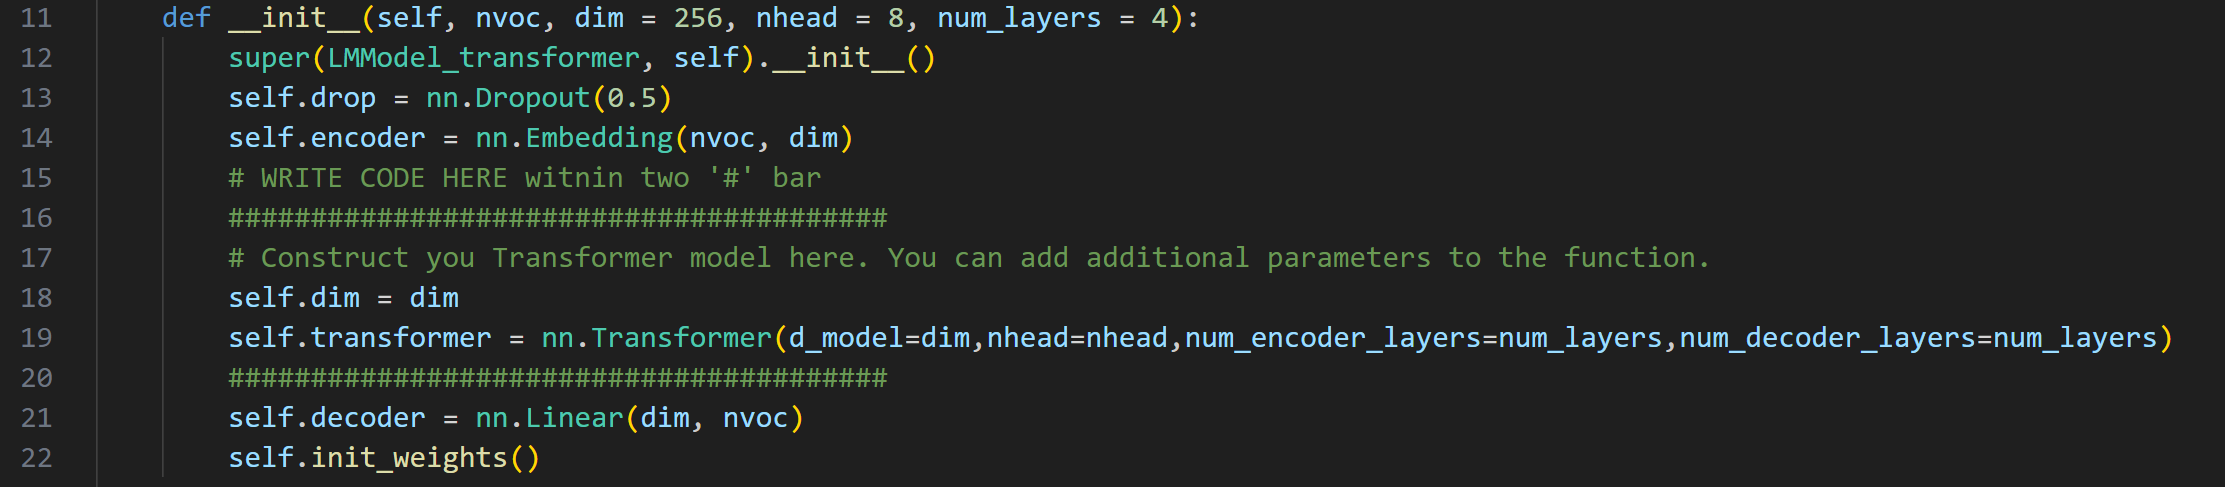
\includegraphics[width=12cm]{code2.png}
  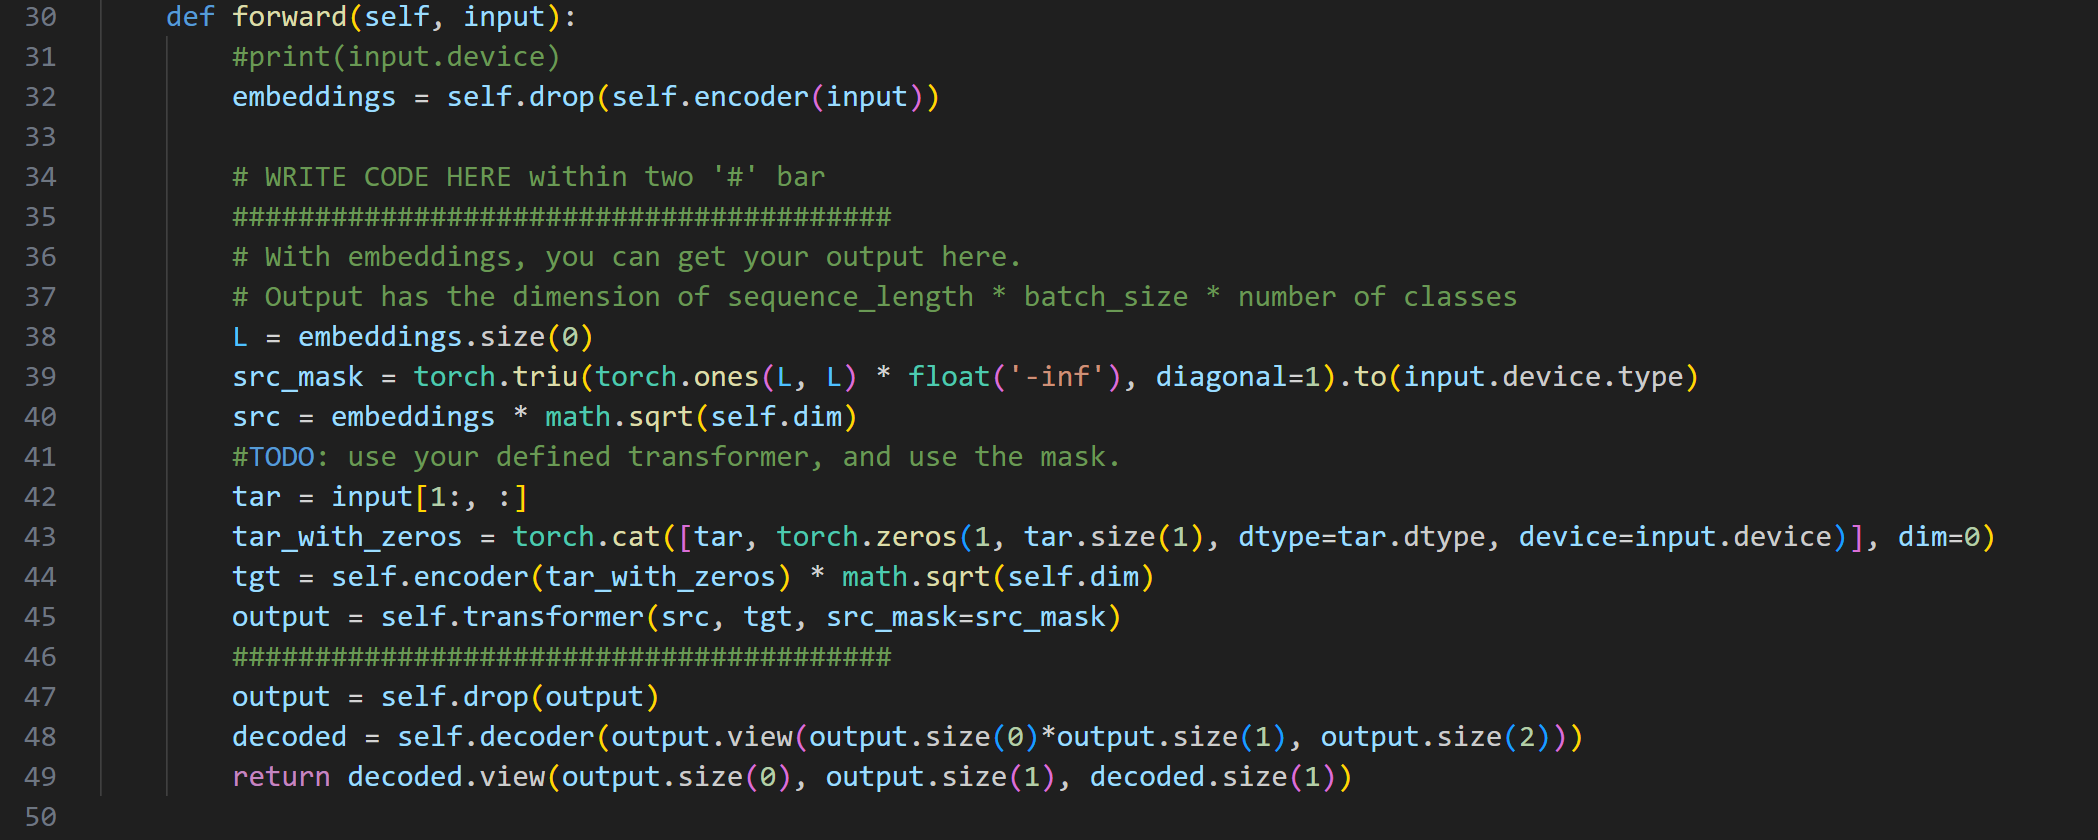
\includegraphics[width=12cm]{code1.png}
\end{figure}
The perplexity curves is shown as below.
\begin{figure}[htbp]
  \begin{center}
    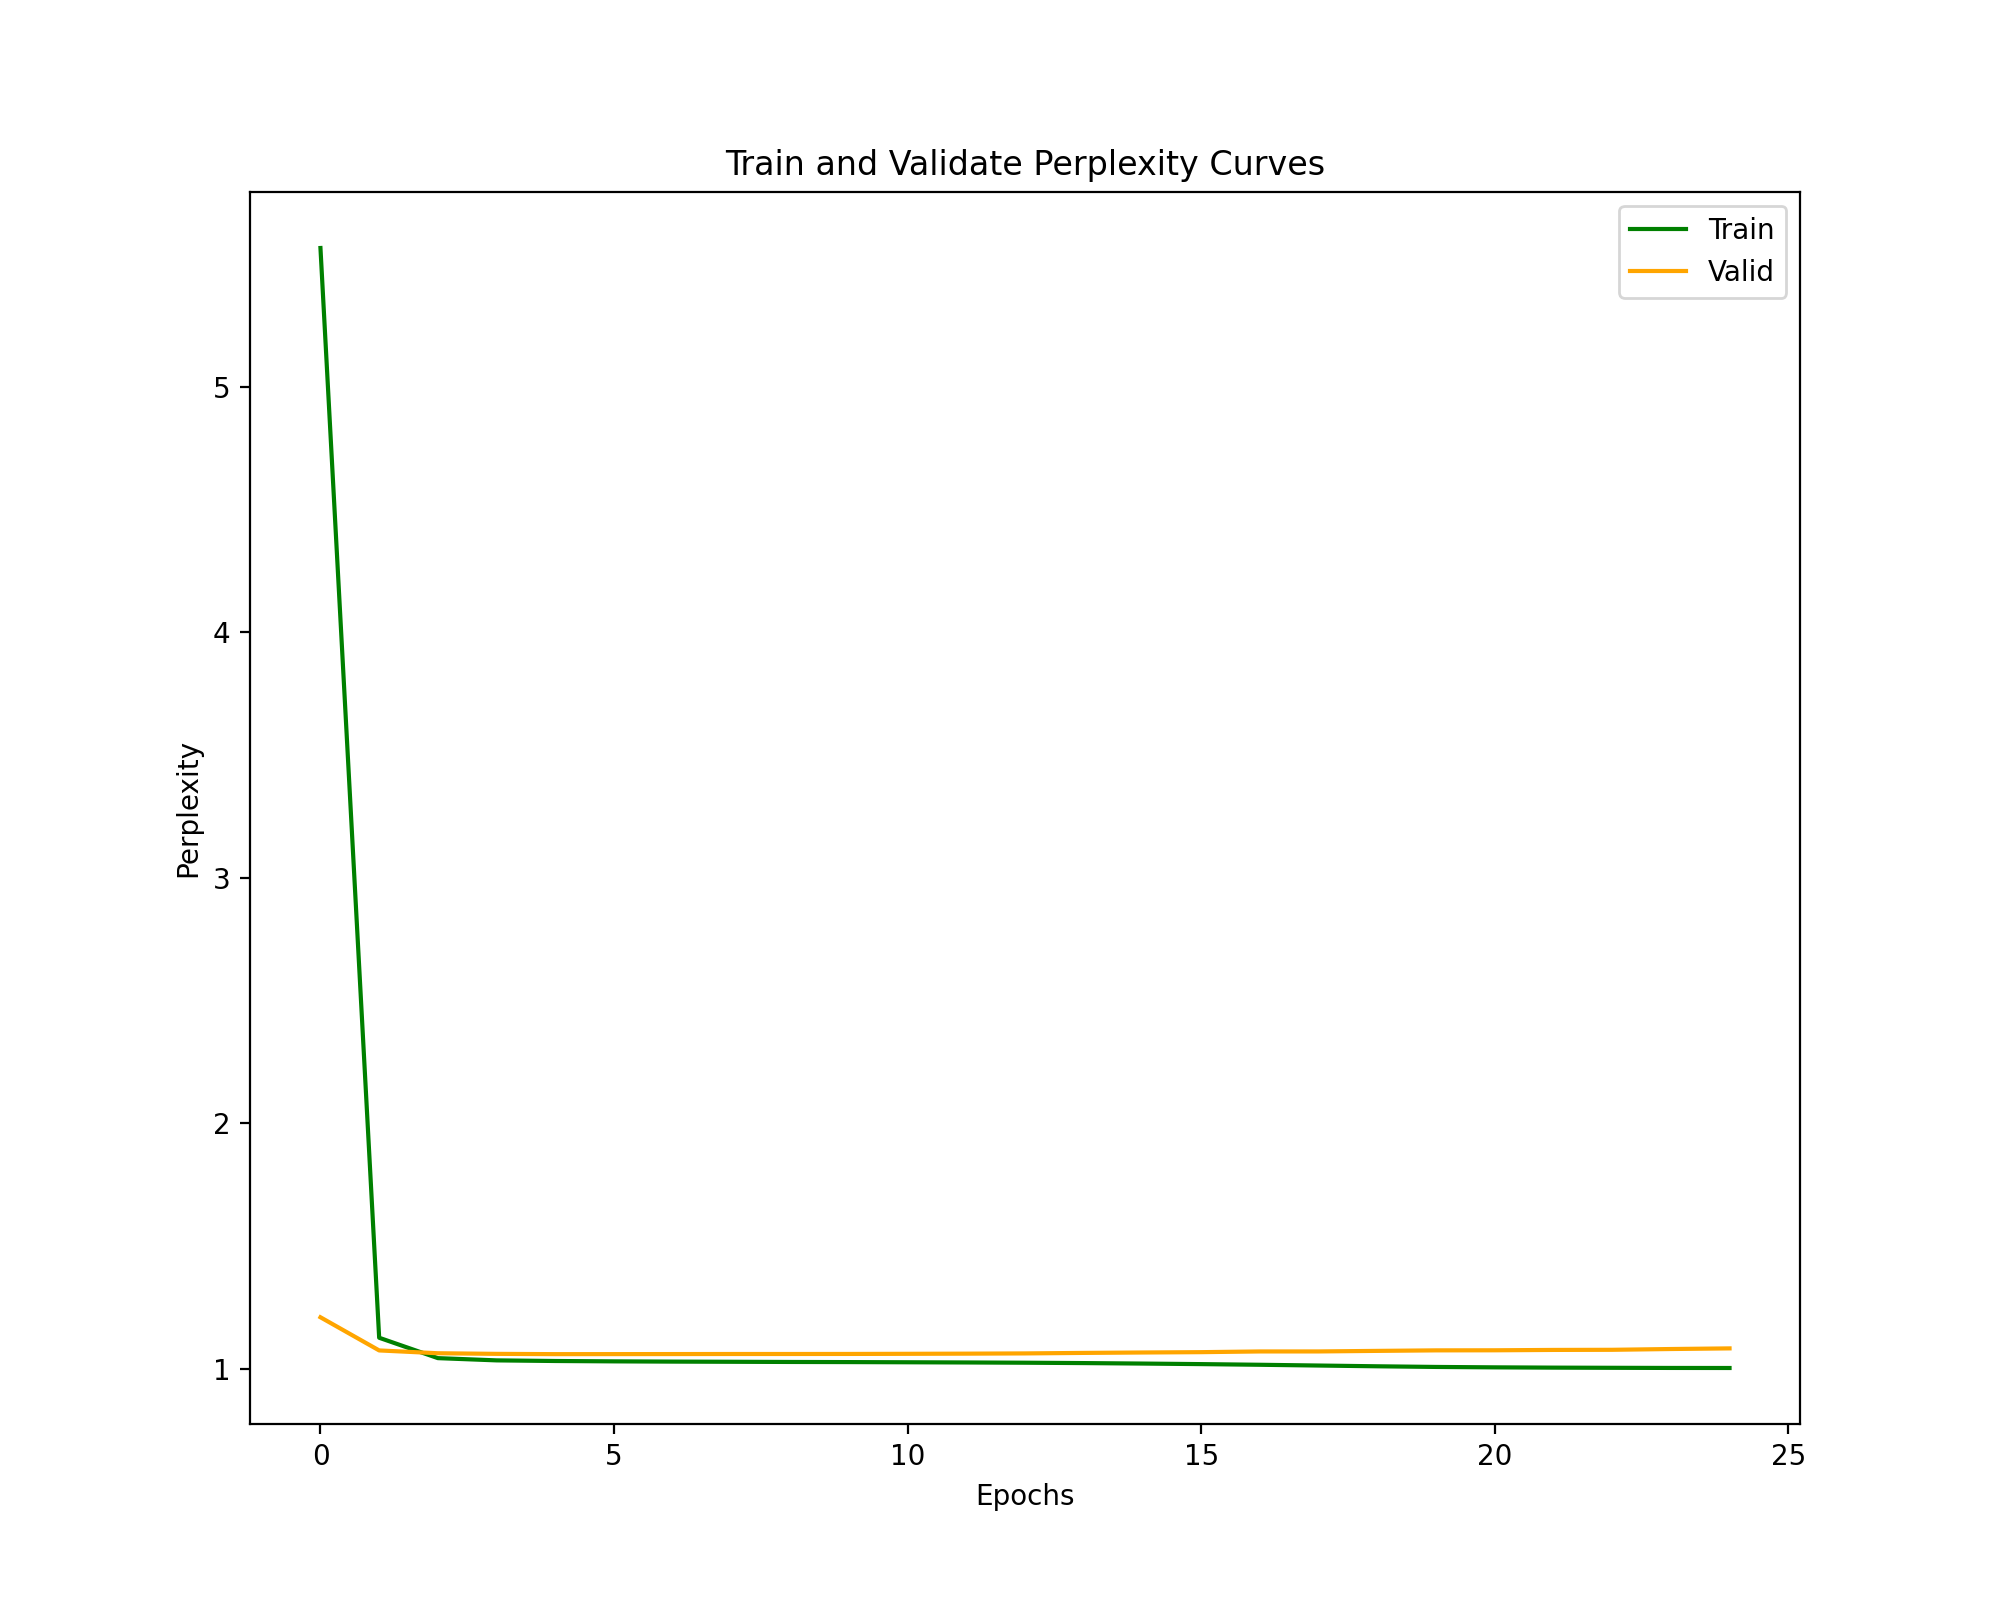
\includegraphics[width=10cm]{per.png}
  \end{center}
\end{figure}

A source mask is a tensor that is used to control the attention mechanism in the transformer. 
It can prevent attention to certain positions or modify the attention weights. 
For example, a source mask can be used to mask out the padding tokens in a sequence or to implement causal 
masking for autoregressive models.

\end{homeworkProblem}

\begin{homeworkProblem}
  Text preprocessing is an essential step to prepare the corpus for modeling and directly affects the natural language processing (NLP) application results. For instance, precise tokenization increases the accuracy of part-of-speech (POS) tagging, and retaining multiword expressions improves reasoning 1.

On the other hand, image preprocessing is used to prepare images for analysis by removing noise, enhancing features, and transforming images into a format that can be easily analyzed by machine learning algorithms.
\end{homeworkProblem}


% \newpage
\Acknowledgement{Thank Yihan Zhou (周亦涵-2020012853) for
the discussion about this homework.}

% End edit to here
%%%%%%%%%%%%%%%%%%%%%%%%%%%%%%%%%%%%%%%%%%%%%%%%%%%%%%%%%%%%%

\end{spacing}
\end{document}

%%%%%%%%%%%%%%%%%%%%%%%%%%%%%%%%%%%%%%%%%%%%%%%%%%%%%%%%%%%%%
